\chapter{操作系统实验环境}

\section{实验目的}
  \begin{enumerate}
    \item 了解操作系统实验的意义
    \item 掌握操作系统实验环境搭建
    \item 了解实验用到的开发工具
  \end{enumerate}
在本章中,我们介绍了一般的linux环境下,操作系统开发的环境搭建的过程,这个过程对不同的操作系统开发,有一定的普适性。
但目前整个实验环境在虚拟机上已经提供,如果无意在本地搭建环境且认为自己足够了解实验意义和相关工具的话,可以跳过这个章节。
    
\section{了解操作系统实验}
关于操作系统的教程可以说是数不胜数,但是对于一个从来没有写过或者参与过操作系统开发的人来说,
这些书读起来总觉得有隔阂,没有一个感性的认识。这其中的根本原因,在于初学者一开始就面对一个完整的操作系统,
或者是面对前人积累了几十年的一系列理论成果(比如经典的页面替换算法)。而这些书的作者无论多擅长写作,或者写的代码多么优秀,
要一个初学者理清其中的头绪都是相当困难的。

操作系统教程中往往注重一些理论知识的讲解,对具体实现的细节描述不够。初学者要是真的想自己动手写一个操作系统,
会发现理论书籍一下子变得毫无用武之地。初学者甚至连如何将一个已经写好的操作系统原型加载到内存中都要花费很长时间,
更不要说自己写出一个比较完善的操作系统。因此,要对操作系统有一个全面的理解,不仅要精读操作系统理论书籍,更要亲自动手编写代码,
只有理论联合实际才能够完全掌握操作系统的精髓所在。

很多国际顶尖的高校为了操作系统的教学,编写了专门的操作系统。JOS是由麻省理工学院教学专用的操作系统,
麻省理工学院的操作系统课程之前一直用的是JOS操作系统,该系统也是在很多学生的努力下完善起来的。这个操作系统实验是MIT公开课中的一个课程,
搭建了一个基础的操作系统框架,让学生一步一步地实现操作系统中的内存管理、中断和异常处理、进程的创建和调度、SMP支持、文件系统等功能,
对于理解操作系统的实现非常有帮助。做完这个实验之后,可以对操作系统的实现有一个整体的、又不失细节的理解。
这个操作系统还有一个特点就是它是一个微内核的系统,如果想要对比宏内核(比如Linux)和微内核,也是一个很不错的选择。
Harvard大学的David A.Holland等也设计了OS161操作系统用于实现操作系统实验教学。因此,我们可以站在巨人的肩膀上,
参考他们的设计思路、方法和源代码,尝试完成一个可以在mips上运行的小型操作系统。
“麻雀虽小,五脏俱全”,在完成这个基于mips架构的小操作系统过程中,我们可以更好的理解操作系统启动、物理内存管理、
虚拟内存管理、进程管理、中断处理、系统调用、文件系统、Shell等主要操作系统内核功能,
每个实验包含的内核代码量(C、汇编、注释)在1000行左右,充分体现了“小而全”的指导思想。

这个基于mips的小操作系统是运行在mips体系结构上的,而我们平常使用的都是基于x86体系结构的计算机,所以为了调试和开发的方便,
我们采用mips硬件模拟器GXEMUL。实验的开发环境是GNU的gcc、gas等工具。整个实验的运行和开发环境都在Linux中。

那么,我们如何来一步步地实现这个基于mips的小操作系统呢?根据一个操作系统和设计实现过程,可以有如下的实验步骤。
\begin{enumerate}
  \item 启动操作系统的bootloader,用于了解操作系统启动前的状态和准备工作,了解运行操作系统的硬件支持,操作系统如何加载到内存中,理解中断等。
  \item 物理内存和虚拟内存管理子系统,理解分段和分页,了解操作系统如何管理物理内存和虚拟内存。
  \item 进程管理和中断管理,了解进程的创建、执行、切换和结束,了解中断的完整过程。
  \item 系统调用,了解系统调用的实现过程。
  \item 文件系统,了解文件系统的具体实现,与进程管理等的关系。
  \item Shell,了解Shell的实现过程。
\end{enumerate}
其中每个开发步骤都是建立在上一个步骤之上,一步一步最终形成一个比较完善的小操作系统,如图\ref{fig:0-1}所示。

\begin{figure}[htbp]
  \centering
  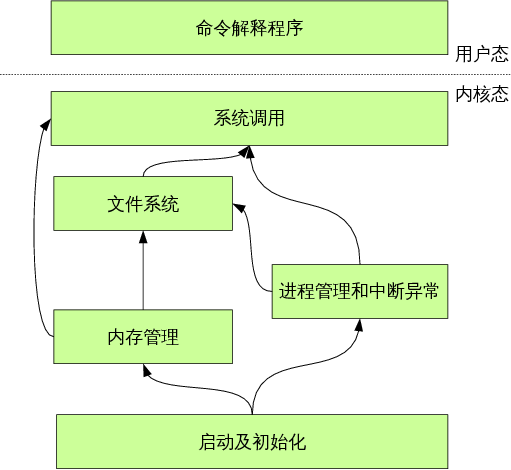
\includegraphics[height=8cm]{0-1}
  \caption{六个实验间的关系}\label{fig:0-1}
\end{figure}

\section{操作系统实验工具}

\subsection{交叉编译器}
首先,整个实验是建立在MIPS上的,通过之前的计算机组成等课程的学习我们知道,不同类型的CPU有不同的ISA。我们本地常使用的是Intel的X86指令集,
或AMD64(EMT64)等指令集。而我们的小操作系统的目标机是MIPS指令集的。但我们需要使用交叉编译器来完成编译过程。
我们的交叉编译器运行于x86平台上,但编译产生的二进制文件却是在mips平台上运行的。如图\ref{fig:0-2}
所示,编译器所运行的平台与其编译出来的程序的平台不同,因此叫做交叉编译器。

\begin{note}
严格意义上来说,所谓平台包含了两个概念:体系结构(Architecture)、操作系统(Operating System)。
一个体系结构上,可以运行多种不同的操作系统。而同一个操作系统,也可以在不同体系结构上运行。
举例来说,我们常说的 x86 Linux 平台实际上是 Intel x86 体系结构和Linux for x86操作系统的统称;
而x86 WinNT平台实际上是Intel x86体系结构和Windows NT for x86 操作系统的简称。
\end{note}

交叉编译器通常用于解决目标平台因性能不足等原因难以直接在其上开发的问题。举个例子,假如我们需要为一个500MHz的ARM开发程序,
因为其性能、工具、环境等原因,我们很难直接在这个ARM的板子上进行开发。因此,我们可以选择在一个性能强劲、工具齐全的x86 PC机上完成程序,
再通过交叉编译器编译为ARM指令集的程序。通过这样的方式,我们就能够轻松地为ARM开发程序了。

\begin{figure}[htbp]
  \centering
  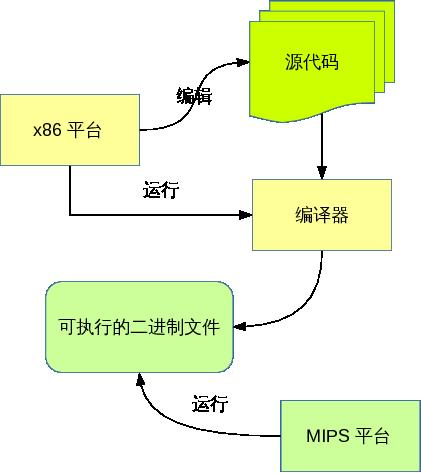
\includegraphics[height=8cm]{0-2}
  \caption{交叉编译}\label{fig:0-2}
\end{figure}

\subsection{Linux系统}
Unix是一个经典的操作系统。目前操作系统中的很多设计思想以及算法均是源自Unix的。
但Unix在商业化后,我们很难以相对廉价的方式直接接触Unix。目前相对较为完善的自由的Unix衍生版仅有FreeBSD等寥寥几个,
其上的软件生态环境等等十分有限。不过,幸运的是,Linux为我们提供了一个相对良好的接触Unix思想的机会。
Linux是一个自由的类Unix(Unix-like)系统,兼容POSIX标准,为我们的实验提供了一个良好的环境。
近些年Linux发展迅猛,其上的软件环境等也十分丰富,这一点相较于BSD家族来说要好很多。
我们实验中采用了GNU的工具,这一套工具主要是为Unix类系统编写的。同时,我们的小操作系统中有很多Unix风格的设计,
因此,采用Linux平台做实验更有利于大家理解实验中的很多内容。实验为大家提供的虚拟机上的环境是一个无图形界面的Ubuntu 12.04,
大家通过ssh远程连接到虚拟机上去做实验。通过命令行界面来进行全部的操作。很多同学以前没有太接触过这种操作方式,这一点需要大家慢慢熟悉。

\begin{note}
事实上,Linux仅仅是一个操作系统内核。一般一个完整的基于Linux的操作系统还包含GNU的各类工具软件,
图形环境,应用软件等等其他一系列的软件。但习惯上,将以Linux为内核的操作系统简称为Linux。
由于大家长期以来习惯在Linux内核上使用大量的GNU软件,所以,Richard Stallman认为将这类操作系统称为“GNU/Linux”更为恰当。
\end{note}

\section{实验环境配置}

\subsection{Linux操作系统}
由于所有的实验都是在Linux下完成的,所以需要Linux操作系统。我们选用设计上更为用户友好的Ubuntu系统。
有两种可供参考的安装方式,一是通过虚拟机来安装Linux系统,二是直接安装Linux系统。这里考虑到大部分同学对于Linux不同熟悉,
我们介绍虚拟机安装的方法。

首先,我们需要下载操作系统的镜像。为了下载速度考虑,我们选择从中国科学与技术大学的镜像站\url{http://mirrors.ustc.edu.cn/}上下载。
点击该页面右侧的\textbf{获取安装镜像},出现如图\ref{fig:get-ubuntu-image}所示的界面,版本选择与实验环境一致的12.04。

\begin{figure}[htbp]
  \centering
  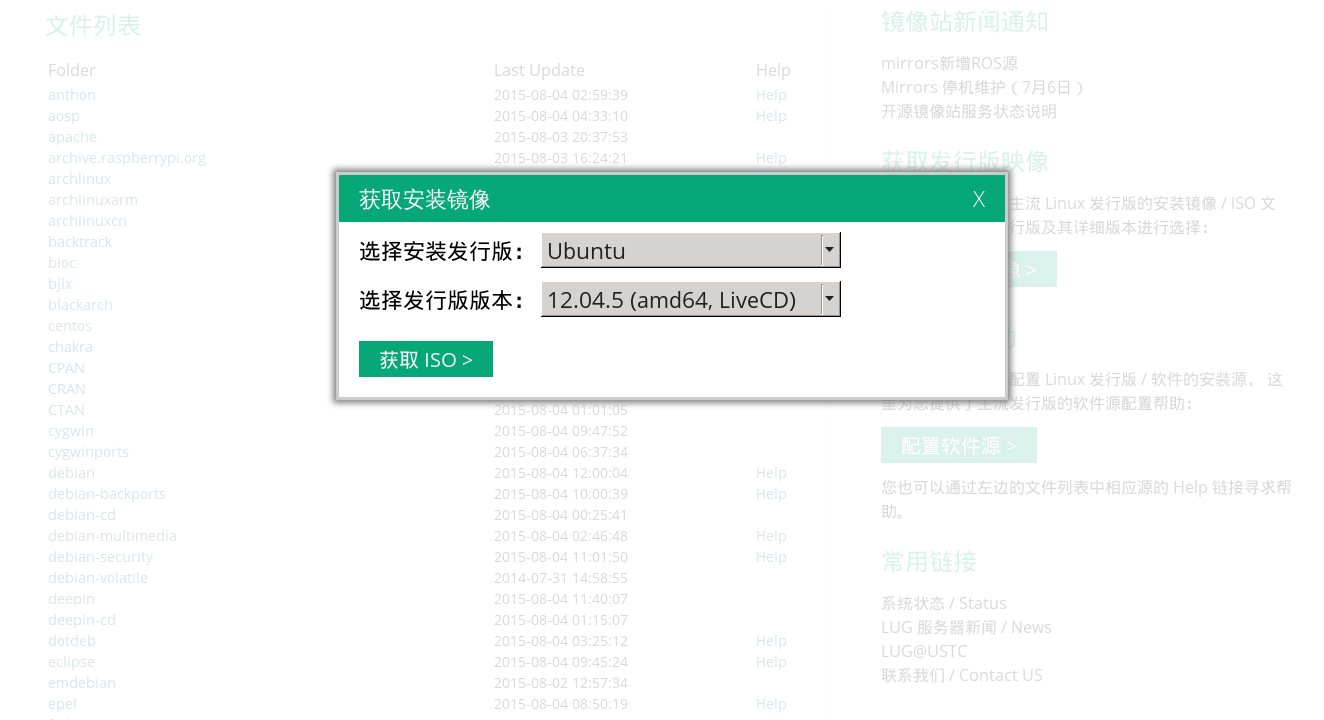
\includegraphics[width=15cm]{get-ubuntu-image}
  \caption{获取安装镜像}\label{fig:get-ubuntu-image}
\end{figure}

接下来,我们下载虚拟机软件。虚拟机相当于一台虚拟的机器,虚拟机上的操作就好像是在操作另一台机器,对本机不会造成影响,
是相对安全的一种体验Linux的方案。这里我们选择采用VirtualBox虚拟机。可以去官网\url{https://www.virtualbox.org/wiki/Downloads}下载,
也可以去百度上自行寻找国内的较快的下载地址。当然,你也可以选择其他的虚拟机软件,如VMware(性能更佳,但是是专有软件,你懂得),具体操作相仿。
但Virtualbox是自由软件,所以出于版权方面的考虑,这里以VirtualBox为例。

安装VirtualBox(相信安装这种小事一定难不住你)后,打开它,看到如图\ref{fig:virtualbox-startup}所示的界面。

\begin{figure}[htbp]
  \centering
  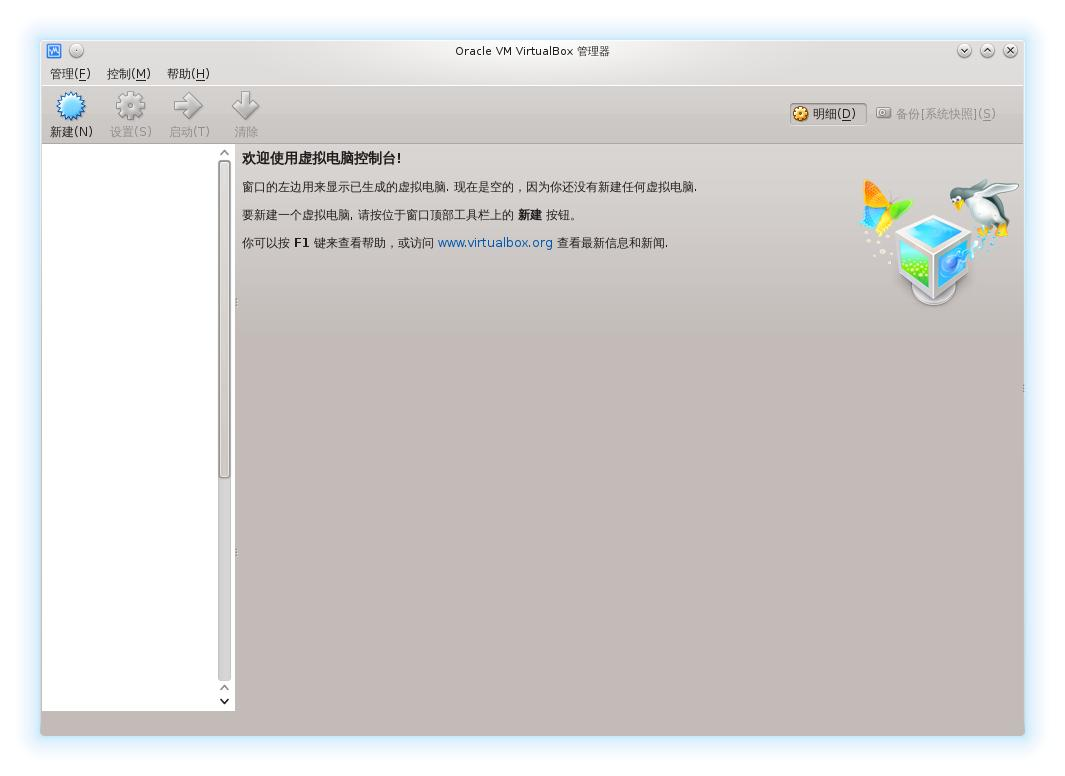
\includegraphics[width=10cm]{virtualbox-startup}
  \caption{VirtualBox虚拟机界面}\label{fig:virtualbox-startup}
\end{figure}

点击\textbf{新建},出现如图\ref{fig:virtualbox-dialog1}所示的对话框。类型选择\textbf{Linux},版本选择\textbf{Ubuntu(64bit)}
(这里如果你下载的时候选择的是i386版本则选择\textbf{Ubuntu(32bit)})。点击\textbf{下一步},内存选择\textbf{1024MB}。
下一步,选择\textbf{现在创建虚拟硬盘},后面的设置如无特殊需求不必改动,一直下一步即可。直到选择磁盘大小处,建议选择\textbf{20GB},
同时选定一个至少有20GB空间的的位置放置磁盘镜像文件。

\begin{figure}[htbp]
  \centering
  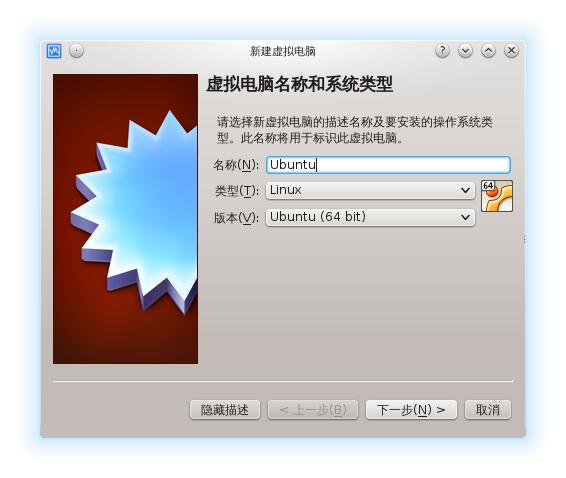
\includegraphics[height=8cm]{virtualbox-dialog1}
  \caption{新建虚拟机}\label{fig:virtualbox-dialog1}
\end{figure}

之后选中我们刚才建立的虚拟机,点\textbf{设置},\textbf{存储},点选\textbf{光盘加号形状图标},\textbf{添加虚拟光驱},
如图\ref{fig:virtualbox-dialog2}然后\textbf{选择磁盘},选中之前下载好的Ubuntu的ISO文件。
      
\begin{figure}[htbp]
  \centering
  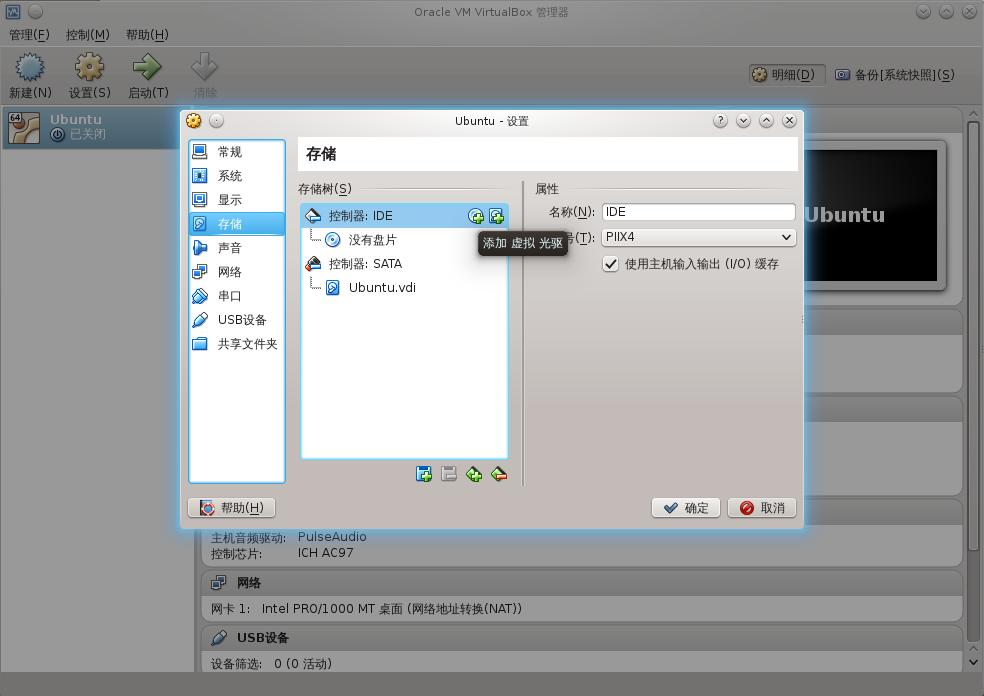
\includegraphics[width=10cm]{virtualbox-dialog2}
  \caption{选择启动镜像}\label{fig:virtualbox-dialog2}
\end{figure}

选中虚拟机,点击\textbf{启动},弹出虚拟机画面,启动后进入Ubuntu的安装界面(见图\ref{fig:ubuntu-install1})。
左侧可以选择语言,这里我们选择\textbf{English},并点击\textbf{Install Ubuntu}。
(当然,按理说选择中文也是没问题的,但这里为了避免任何不必要的麻烦,我们选择了英文)。

\begin{figure}[htbp]
  \centering
  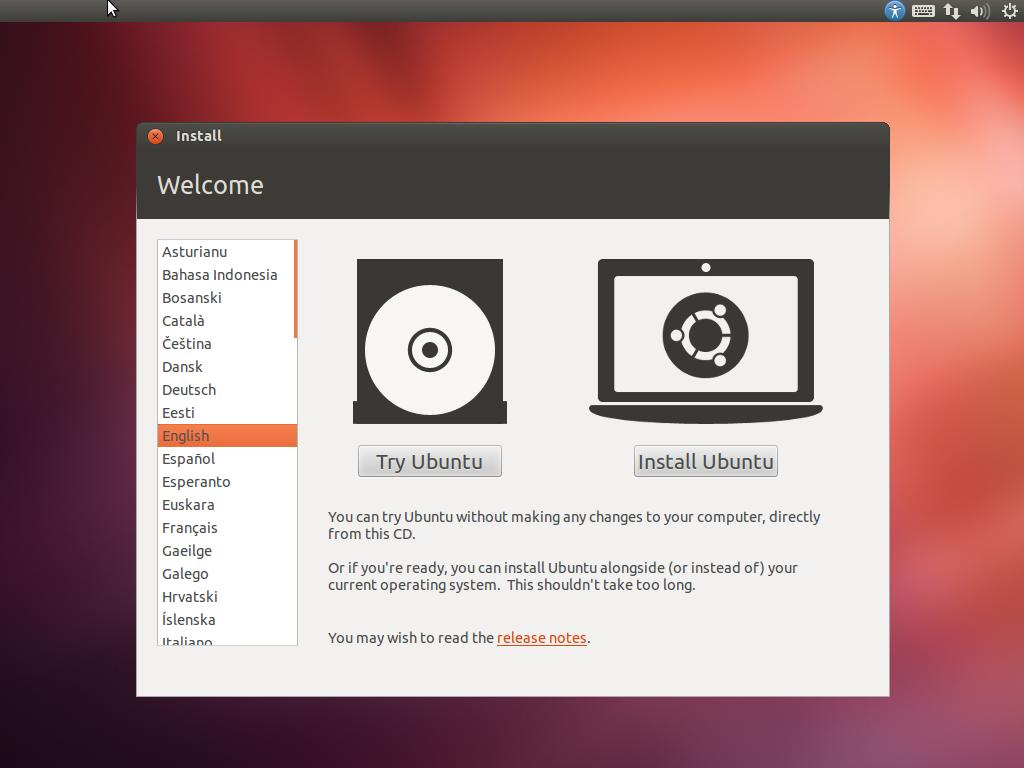
\includegraphics[width=10cm]{ubuntu-install1}
  \caption{选择启动镜像}\label{fig:ubuntu-install1}
\end{figure}

之后由于我们没有改镜像源等设置,为了安装速度考虑,不要选择\textbf{Download updates while installing}。以免Ubuntu
从缓慢的官方服务器下载更新。\textbf{Install this third-party software}选项与我们实验无关,你可以自行选择是否勾选。
下一步选择\textbf{Erase disk and install Ubuntu}。由于我们是在虚拟机上安装,且使用了新建的虚拟磁盘,所以自然可以大胆
地让Ubuntu清空整个磁盘并安装。下一步一般不需要做改动,点击\textbf{Install Now}就好。之后输入密码,等待安装结束就好。

\begin{figure}[htbp]
  \centering
  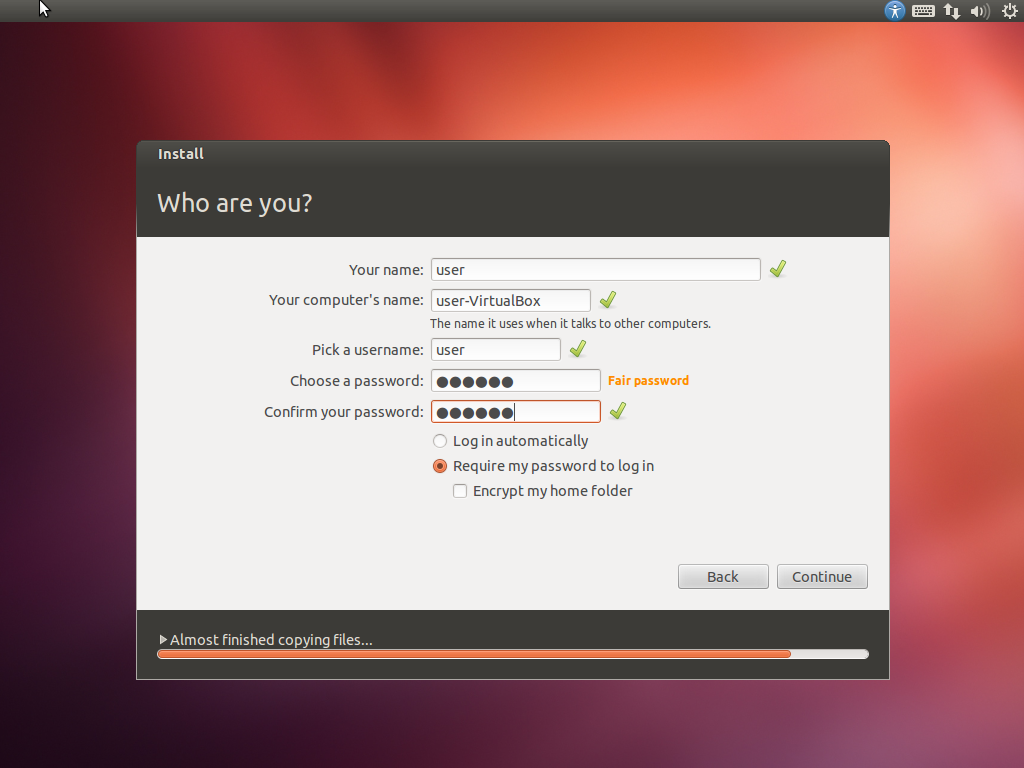
\includegraphics[width=10cm]{ubuntu-install2}
  \caption{Ubuntu安装中新建用户的界面}\label{fig:ubuntu-install2} 
\end{figure}

安装结束后点击\textbf{Restart}重启。重启时注意,安装镜像关闭时一般会提示你取出光盘并按回车键。
光盘镜像正常情况下会被自动弹出。
一般来说,你需要做的仅仅是按下回车键并等待重启。
这里注意,有时候由于种种原因它不会输出这句提示,遇到这种情况就需要发动你的第六感了:)感觉系统不再动了以后敲一个回车就好。

重启完成后登入Ubuntu界面,接下来我们安装增强功能。点击虚拟机的\textbf{设备},然后选择\textbf{安装增强功能}。
之后会Ubuntu会选择弹出对话框询问是否自动运行,如图\ref{fig:ubuntu-install3}所示。点击\textbf{Run}后会
弹出对话框要求输入密码,输入密码后会启动一个命令行,开始执行安装脚本,看到\textbf{Press Return to close this window}
后按回车键结束安装。手动重启虚拟机,重启后虚拟机的分辨率会变成相对正常的状态,说明增强功能已经成功安装。

\begin{figure}[htbp]
  \centering
  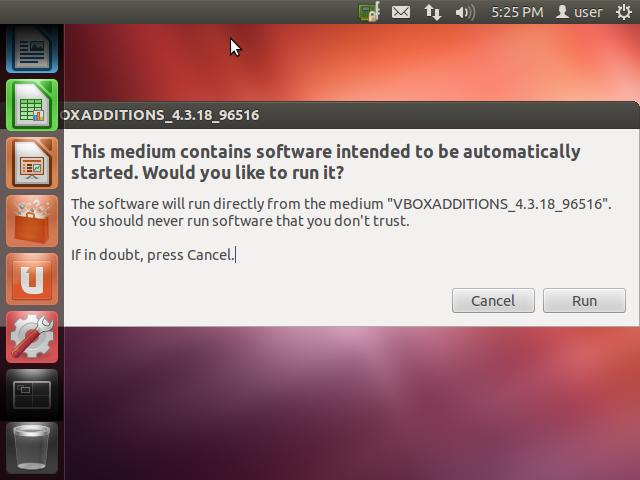
\includegraphics[width=8cm]{ubuntu-install3}
  \caption{Ubuntu安装中新建用户的界面}\label{fig:ubuntu-install3} 
\end{figure}

至此,一个Ubuntu环境就搭建完成了。你可以在上面学习并熟悉Linux的相关指令,并编写我们的实验代码。

\begin{exercise}
安装一个Linux环境,并尝试学会使用ls、cat、cd、cp、mv这五条指令
\end{exercise}

\subsection{安装交叉编译器}
交叉编译器的下载可以访问\url{http://ftp.sunet.se/pub/Linux/distributions/eldk/4.1/mips-linux-x86/iso/}
到其中下载\textbf{mips-2007-01-21.iso}文件。这里下载网速较慢,建议大家下载完一份后相互拷贝,
一般课程中心也会提供相应的文件。

在Ubuntu下,按住Ctrl+Alt+t快捷键,可以打开一个终端,我们在终端中

\begin{minted}[linenos]{bash}
# 建立一个用于挂载ISO镜像的目录
sudo mkdir /mnt/mipsiso
# 挂载iso文件
sudo mount -o loop mips-2007-01-21.iso /mnt/mipsiso
# 切换到/mnt/mipsiso文件夹中
cd /mnt/mipsiso
# 安装32位运行库(仅在64位系统上需要执行此步骤)
sudo apt-get install ia32-libs
# 运行安装脚本
sudo ./install -d /opt/eldk
\end{minted}

执行完上面的指令后,检查/opt/eldk/usr/bin下是否有以mips\_4KC开头的一系列工具。
打开命令行,尝试运行其中的gcc,如果看到如下输出,则说明一切OK~

\begin{minted}[linenos]{bash}
# 注意,此时需要位于/opt/eldk/usr/bin目录下
$ ./mips_4KC-gcc
Reading specs from /opt/eldk/usr/bin/../lib/gcc/mips-linux/4.0.0/specs
Target: mips-linux
Configured with: /opt/eldk/build/mips-2007-01-21/work/usr/src/denx/
BUILD/crosstool-0.35/build/gcc-4.0.0-glibc-2.3.5-eldk/mips-linux/
gcc-4.0.0/configure --target=mips-linux --host=i686-host_pc-linux-gnu 
--prefix=/var/tmp/eldk.PyrfxY/usr/crosstool/gcc-4.0.0-glibc-2.3.5-eldk
/mips-linux --with-headers=/var/tmp/eldk.PyrfxY/usr/crosstool/gcc-4.0.
0-glibc-2.3.5-eldk/mips-linux/mips-linux/include --with-local-prefix=
/var/tmp/eldk.PyrfxY/usr/crosstool/gcc-4.0.0-glibc-2.3.5-eldk/
mips-linux/mips-linux --disable-nls --enable-threads=posix 
--enable-symvers=gnu --enable-languages=c,c++ --enable-shared 
--enable-c99 --enable-long-long --enable-__cxa_atexit
Thread model: posix
gcc version 4.0.0 (DENX ELDK 4.1 4.0.0)
\end{minted}

\subsection{安装仿真器}
由于实验的操作系统内核是运行在mips体系结构上的,而我们平常使用的是基于x86体系结构的PC,
所以需要使用仿真器来仿真一个mips体系结构的环境,来让我们的操作系统内核运行。在这个实验中我们使用的是 gxemul 仿真器。

我们需要从\url{http://gxemul.sourceforge.net/src/}下载gxemul-0.4.6.tar.gz。
这里需要注意,一定要下载0.4系列的gxemul,而不是最新的0.6系列,以免发生和实验提供的文件发生不兼容的现象。
调出终端,切换到gxemul-0.4.6.tar.gz所在目录,执行以下指令

\begin{minted}[linenos]{bash}
# 解压gxemul-0.4.6.tar.gz
tar -zxvf gxemul-0.4.6.tar.gz
# 进入gxemul文件夹
cd gxemul-0.4.6
# 配置并编译安装
./configure
make
sudo make install
sudo cp gxemul /usr/local/bin
\end{minted}

在命令行中执行gxemul指令,看到如下输出则说明gxemul安装正确。

\begin{minted}[linenos]{bash}
$ gxemul
GXemul 0.4.6    Copyright (C) 2003-2007  Anders Gavare
Read the source code and/or documentation for other Copyright messages.

usage: gxemul [machine, other, and general options] [file [...]]
   or  gxemul [general options] @configfile
   or  gxemul [userland, other, and general options] file [args ...]

Run  gxemul -h  for help on command line options.

No filename given. Aborting.
\end{minted}

\begin{exercise}
安装交叉编译器及gxemul,并确认其正常运行。
\end{exercise}

\section{实验思考}

\begin{thinking}
思考以下几条指令有何作用?
  \begin{itemize}
    \item ls -l
    \item mv test1.c test2.c
    \item cp test1.c test2.c
    \item cd ..
  \end{itemize}
\end{thinking}
我们的整个实验环境全部是运行于Linux基础上的,且所提供的虚拟机是没有安装图形界面的,需要通过ssh远程连接访问。
实验的所有操作全部在命令行下完成。因此,在开始实验前,你需要掌握最基本的一些命令,以保证你可以\textbf{在命令行下生存}

\begin{thinking}
思考grep指令的用法,例如如何查找项目中所有的宏?如何查找指定的函数名?
\end{thinking}
grep指令可以在文件中\textbf{匹配特定的文本}。支持递归匹配(即查找当前目录及子目录下所有文件)、正则表达式等一系列有用的功能。
当你需要在整个项目目录中查找某个函数名、变量名等等的时候,grep将是你手头一个强有力的工具。
这里给一个提示,grep的-a、-i、-r三个选项使用率较高,可以着重了解一下。

\begin{thinking}
思考gcc的-Werror和-Wall两个参数在项目开发中的意义。
\end{thinking}
编译器警告很多时候可以帮你发现一些代码上的错误。善用编译器警告可以大大加快你调试的进度。
